%%%% Full manuscript draft — IJCAI--ECAI 26 (two-column).
%%%% Build: pdflatex yoruba_ocr && bibtex yoruba_ocr && pdflatex x2

\typeout{Yoruba OCR — IJCAI--ECAI 26 draft}

\documentclass{article}
\pdfpagewidth=8.5in
\pdfpageheight=11in

\usepackage{ijcai26}
\usepackage{times}
\usepackage{soul}
\usepackage{url}
\usepackage[hidelinks]{hyperref}
\usepackage[utf8]{inputenc}
\usepackage[small]{caption}
\usepackage{graphicx}
\usepackage{amsmath}
\usepackage{amsthm}
\usepackage{booktabs}
\usepackage{algorithm}
\usepackage{algorithmic}
\usepackage[switch]{lineno}
\usepackage{xcolor}

\linenumbers

\urlstyle{same}

\newcommand{\Yoruba}{Yor\`ub\'a}
\newcommand{\TODO}[1]{\textcolor{red}{[TODO: #1]}}

\newtheorem{definition}{Definition}

\pdfinfo{
/TemplateVersion (IJCAI.2026.0)
}

\title{Faithful \Yoruba{} OCR: A Diacritic-Sensitive Benchmark Revealing Failure Modes in Multimodal OCR}

\author{
Anonymous Authors
}

\begin{document}

\maketitle

%% ============================================================
%% ABSTRACT
%% ============================================================
\begin{abstract}
Optical Character Recognition (OCR) for African languages remains underdeveloped, especially for tone languages such as \Yoruba{}, where diacritics are semantically contrastive. For example, the base syllable sequence \emph{igba} maps to five unrelated words depending solely on tonal marking: \emph{igba} (two hundred), \emph{igb\'a} (calabash), \emph{\`igb\`a} (season/time), \emph{\`igb\'a} (garden egg), and \emph{igb\`a} (a type of rope). Widely deployed OCR engines and multimodal large language models (MLLMs) frequently confuse such diacritic minimal sets, yielding outputs that alter meaning.
We introduce a curated corpus of 2{,}945 human-corrected line crops from the six-volume \emph{\Yoruba{} di W\'ur\`a} graded reader series, merged into a single corpus with export-stable train/validation/test partitions (2{,}367 / 252 / 326 lines; Table~\ref{tab:split}). We benchmark classical OCR, vision-language models (VLMs), and Qwen~2.5-VL-3B zero-shot, and we propose \emph{Diacritic Error Rate} (DER) to isolate tone-mark errors from base-character corruption.
We find that even with targeted LoRA fine-tuning, the best-performing model (PaddleOCR-VL-1.5) still misrecognizes roughly two-thirds of combining diacritics on the held-out test split (corpus DER${=}66.4\%$ over $n_{\mathrm{der}}{=}319$ diacritic-bearing lines), exposing a fundamental evaluation blind spot. While MLLMs sometimes infer correct words from context, they suffer from graphemic hallucinations. Our benchmark provides a diagnostic tool to measure this fidelity gap, demonstrating that current architectures remain inadequate for archival digitization of tonal scripts. Data and code will be publicly released.
\end{abstract}

%% ============================================================
%% 1. INTRODUCTION
%% ============================================================
\section{Introduction}

The digitization of African-language texts remains a bottleneck for natural language processing (NLP) on the continent. OCR has reached near-human accuracy for high-resource languages~\cite{du2020ppocr}, yet low-resource tonal languages -- particularly those with complex diacritic systems -- remain severely underserved~\cite{agarwal2024ocr}.

\Yoruba{}, spoken by over 50 million people in West Africa, presents a particularly acute challenge. The language employs a three-tone system (high, mid, low) encoded orthographically through acute, grave, and unmarked conventions on vowels and the syllabic nasal. These diacritics are semantically contrastive. Consider the base syllable sequence \emph{igba}: \emph{igba} means `two hundred' (mid-mid), \emph{igb\'a} means `calabash' (mid-high), \emph{\`igb\`a} means `season/time' (low-low), \emph{\`igb\'a} means `garden egg' (low-high), and \emph{igb\`a} means `a type of rope' (mid-low). A system that drops or misreads a single tone mark does not degrade the transcription -- it produces a semantically different word.

Standard metrics such as Character Error Rate (CER) and Word Error Rate (WER) treat all substitutions equally. A system that transcribes \emph{\`e} as \emph{e} incurs the same penalty as one that substitutes an entirely unrelated character, obscuring the failure mode most damaging for \Yoruba{}: the systematic dropping of diacritics.

This paper addresses three gaps: the absence of a linguistically validated \Yoruba{} OCR benchmark, the lack of systematic MLLM evaluation on \Yoruba{} text recognition~\cite{sohail2024deciphering}, and the insensitivity of existing metrics to tonal error patterns.

We make three contributions: \textbf{(i)}~to our knowledge, the first diacritic-faithful OCR benchmark for \Yoruba{}, featuring human-corrected line-image annotations from a merged six-volume corpus (2{,}367 / 252 / 326 export-stable split); \textbf{(ii)}~\emph{Diacritic Error Rate} (DER), a linguistically grounded evaluation metric for tonal scripts; and \textbf{(iii)}~empirical evidence that modern VLMs fail at graphemic fidelity, revealing an evaluation blind spot where current architectures fall short. All data and code will be publicly released.

%% ============================================================
%% 2. RELATED WORK
%% ============================================================
\section{Related Work}

\paragraph{OCR for low-resource scripts.}
Industrial OCR pipelines converge on detection-recognition architectures achieving strong accuracy on Latin, CJK, and Arabic scripts~\cite{du2020ppocr,du2021ppocrv2,smith2007tesseract}. PaddleOCR recently introduced a 0.9B-parameter vision-language variant~\cite{cui2026paddleocrvl}; Tesseract remains widely deployed through open-source language packs. Both are benchmarked on high-resource corpora where diacritics are absent or non-contrastive; African tonal scripts are rarely primary targets. A recent survey~\cite{agarwal2024ocr} identifies data scarcity and script complexity as persistent barriers for low-resource OCR, while Sohail et~al.~\shortcite{sohail2024deciphering} benchmark LLM-based OCR on underserved scripts.

\paragraph{Diacritic handling in NLP.}
Diacritic restoration has been studied for Arabic, Vietnamese, and European languages. For \Yoruba{}, Orife~\shortcite{orife2018adr} applied attentive sequence-to-sequence models to restore diacritics from unaccented text, and Adelani et~al.~\shortcite{adelani2015diacritics} proposed improvements using pre-trained embeddings. Both assume clean text as input, side-stepping the compounded difficulty of recognizing diacritics from noisy pixel data. The interaction between OCR recognition errors and diacritic fidelity remains unquantified.

\paragraph{African-language NLP resources.}
Cross-lingual corpora have primarily targeted downstream NLP tasks. MasakhaNER~\cite{adelani2021masakhaner} established named entity benchmarks across African languages; AfriSenti~\cite{muhammad2023afrisenti} expanded to sentiment analysis. OCR complements these efforts: scanned pedagogical texts are a major data source if diacritically faithful transcriptions can be recovered. To our knowledge, no prior work releases a \Yoruba{} line-OCR benchmark with diacritic-aware evaluation.

\paragraph{Vision-language models for document understanding.}
MLLMs such as Qwen2-VL~\cite{bai2024qwen2vl} and its successor Qwen~2.5-VL~\cite{qwen2025vl} report strong document parsing on English-centric suites. PaddleOCR-VL-1.5~\cite{cui2026paddleocrvl} targets document OCR with a compact 0.9B architecture. Their behaviour on low-resource orthographies with contrastive diacritics is under-studied. A key question is whether contextual reasoning compensates for graphemic errors or introduces a different class of unfaithful transcription.

%% ============================================================
%% 3. YORUBA ORTHOGRAPHY & PROBLEM FORMULATION
%% ============================================================
\section{\Yoruba{} Orthography and Problem Formulation}

Standard \Yoruba{} orthography employs a Latin-based script augmented with three classes of diacritical marks. Tone is marked on vowels (a, e, \d{e}, i, o, \d{o}, u) and the syllabic nasal using acute accent for high tone, grave accent for low tone, and no marking for mid tone. Sub-dot diacritics distinguish open vowels (\d{e}/e and \d{o}/o) and the consonant \d{s}/s. These marks interact multiplicatively: a single vowel may carry both a sub-dot and a tone accent (e.g., \d{o}\kern-0.15em\`{}, \d{e}\kern-0.15em\'{}).

The realization of low-tone diacritics on the syllabic nasals /n/ and /m/ exhibits particular sensitivity: misalignment between tonal marking and the tone-bearing unit (TBU) is a common OCR failure mode. Similarly, high-tone diacritics on /m/ are frequently misplaced, reflecting inconsistencies in how OCR systems model the orthographic representation of tone.

Let $\Sigma$ denote the Standard \Yoruba{} character set, with $|\Sigma|{=}99$ after NFC normalization. Each label is a string $y \in \Sigma^\ast$ aligned to a text-line image $x$. The task is sequence transcription: predict $\hat{y}$ minimizing edit distance to $y$.

Let $\mathcal{U} \subset \Sigma$ denote codepoints that participate in tonal or sub-dot contrasts. In the curated corpus, combining diacritics comprise 28{,}956 instances (11{,}248 combining acute, 9{,}328 combining grave, 8{,}380 combining dot below) alongside 24{,}308 precomposed diacritic characters. Errors on $\mathcal{U}$ drive DER (\S\ref{sec:der}).

%% ============================================================
%% 4. DATASET
%% ============================================================
\section{Dataset}

\paragraph{Source material.}
Line crops originate from the \emph{\Yoruba{} di W\'ur\`a} graded reader series (Books~1--6)~\cite{oyedele2020ydw}, professionally typeset educational material with verified ground truth with known typographic properties.

\paragraph{Annotation pipeline.}
We built a custom web-based annotation platform (\emph{\Yoruba{} OCR Hub}, Figure~\ref{fig:interface}) to streamline data collection. Page scans were uploaded and segmented at line granularity. An embedded PaddleOCR-VL-1.5 model~\cite{cui2026paddleocrvl} generated initial transcription hypotheses for each line crop. Two annotators fluent in \Yoruba{} then manually reviewed and corrected every prediction, paying particular attention to tonal diacritics that the automated system consistently misrecognized. A number of revised forms were automatically normalized by the software; for example, \textsc{\'AK\'IY\`ES\'I} was system-generated following successive iterations of manual correction, reflecting post-editing intervention by the text-processing algorithm. All transcriptions were normalized to UTF-8 NFC form. The pipeline processed 33 independent export batches, consolidated and deduplicated programmatically.

\begin{figure}[t]
  \centering
  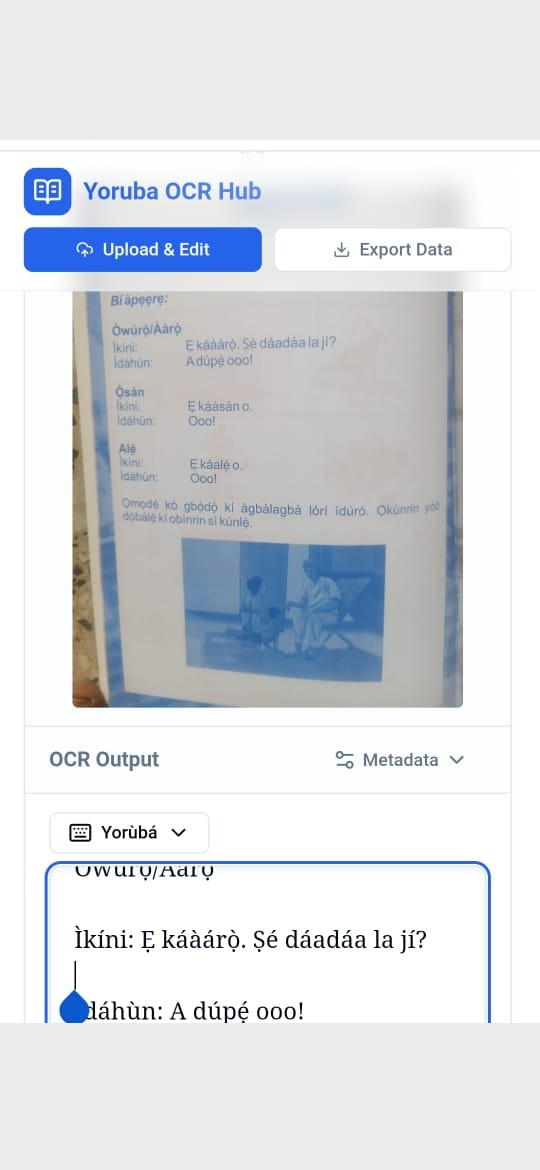
\includegraphics[width=0.95\columnwidth]{figures/ocr_extraction_interface.jpeg}
  \caption{The annotation interface (browser chrome redacted for anonymous review). Top: scanned page from \emph{\Yoruba{} di W\'ur\`a}. Bottom: OCR output with embedded \Yoruba{} keyboard for manual diacritic correction by annotators.}
  \label{fig:interface}
\end{figure}

\paragraph{Data hygiene.}
A filter removed labels shorter than 3 or longer than 100 characters, lines containing non-\Yoruba{} codepoints, and entries flagged as invalid. Specifically: 640 invalid entries, 386 non-whitelisted codepoints, 348 labels too short, and 236 too long were excluded. The resulting dataset comprises \textbf{2{,}945 unique line crops}.

\paragraph{Train/validation/test split.}
All six \emph{\Yoruba{} di W\'ur\`a} volumes are merged into one corpus of
2{,}945 unique line crops after hygiene filtering. We did \textbf{not} apply
the optional \texttt{--resplit} pass: every model in this paper is trained and
evaluated on \textbf{export-stable} partitions preserved from the annotation
platform (\texttt{split\_source=on\_disk\_labels} in
\texttt{consolidation\_report.json}): \textbf{2{,}367 train / 252 validation /
326 test} lines. Table~\ref{tab:main} and all auxiliary analyses use the
326-line \emph{test} split only; VL-1.5 LoRA trains on the 2{,}367-line train
split (validation held out for monitoring). Table~\ref{tab:split} contrasts
this policy with an optional 80/10/10 line-level reassignment
(\texttt{--resplit --seed 42}), which we document for reproducibility but do
not use for any reported score.

\begin{table}[t]
  \centering
  \small
  \begin{tabular}{llrrr}
    \toprule
    Split policy & Used in paper? & Train & Val & Test \\
    \midrule
    Export-stable (platform batches) & \textbf{Yes} & 2{,}367 & 252 & 326 \\
    Optional 80/10/10 (\texttt{--resplit --seed 42}) & No & 2{,}356 & 294 & 295 \\
    \bottomrule
  \end{tabular}
  \caption{Train/validation/test partitions for the merged 2{,}945-line corpus.
  \textbf{All experiments}---PP-OCRv4 ablations, Tesseract baselines,
  PaddleOCR-VL-1.5 zero-shot/LoRA, and archived MLLM pilots---use the
  export-stable row. Re-running with \texttt{--resplit} changes line counts and
  requires re-evaluating every system.}
  \label{tab:split}
\end{table}

\paragraph{Character dictionary.}
The dictionary contains \textbf{99 unique characters} (excluding space), closed under NFC normalization. It covers all tonal vowel variants, sub-dotted vowels and consonants, uppercase variants, digits, and common punctuation. Coverage of in-distribution text is 99.0\%.

\paragraph{Dataset scale vs.\ quality.}
While a corpus of 2{,}945 lines is modest compared to synthetic high-resource OCR datasets, line-level annotated data for African languages is exceptionally rare. We prioritized annotation quality -- specifically human correction of every tonal diacritic -- over scraped volume. This ensures the benchmark measures true graphemic fidelity rather than dataset noise.

%% ============================================================
%% 5. MODELS AND TRAINING
%% ============================================================
\section{Models and Training}

Table~\ref{tab:models} summarizes the evaluated systems, their parameter counts, and architecture types.

\begin{table}[t]
  \centering
  \small
  \begin{tabular}{lrll}
    \toprule
    System & Params & Type & Adaptation \\
    \midrule
    PP-OCRv4$^\dagger$ & ${\sim}$11M & CRNN+CTC & Fine-tuned \\
    Tesseract~5 & -- & LSTM+CTC & Zero-shot \\
    VL-1.5 & 0.9B & VLM & Zero-shot \\
    VL-1.5 (LoRA) & 0.9B & VLM & LoRA r=16 \\
    Qwen 2.5 VL-3B & 3B & MLLM & Zero-shot \\
    Surya v2$^\ddagger$ & 0.9B & VLM & Zero-shot \\
    TrOCR-large-printed$^\ddagger$ & 334M & Enc--Dec & Fine-tuned \\
    \bottomrule
  \end{tabular}
  \caption{Systems evaluated. ``Params'' denotes total model parameters. Tesseract model size is not publicly disclosed. $^\dagger$PP-OCRv4 metrics appear in data-size ablation (Table~\ref{tab:ablation}) from an archived evaluation; training checkpoints were not on disk at paper freeze and the row is omitted from Table~\ref{tab:main}. $^\ddagger$Surya and TrOCR are implemented in the release pipeline but not included in Table~\ref{tab:main} for this submission.}
  \label{tab:models}
\end{table}

\paragraph{PaddleOCR PP-OCRv4.}
We fine-tuned the English-pretrained PP-OCRv4 recognition model~\cite{du2020ppocr} (${\sim}$11M parameters, SVTR\_LCNet with CTC head) on the full training split for 40 epochs with Adam, cosine lr schedule (lr=0.001), RecAug augmentation, and our 99-character \Yoruba{} dictionary.

\paragraph{Tesseract.}
Tesseract~5~\cite{smith2007tesseract} was evaluated under three language configurations: English (\texttt{eng}), \Yoruba{} (\texttt{yor}), and combined (\texttt{eng+yor}), all with default parameters.

\paragraph{Qwen 2.5 VL.}
\label{sec:models-qwen}
We evaluate \texttt{Qwen/Qwen2.5-VL-3B-Instruct}~\cite{qwen2025vl,bai2024qwen2vl}
zero-shot with a fixed instruction template and temperature~0
(\texttt{scripts/09\_baseline\_qwen.py}; 4-bit quantisation on NVIDIA T4).
Table~\ref{tab:main} omits the MLLM row until 3B metrics are logged under
\texttt{qwen25\_vl3\_zero\_shot}; an archived \texttt{Qwen2.5-VL-7B-Instruct}
pilot on the same export-stable test split (CER 253.5\%, DER 119.6\%) is
discussed qualitatively below.

\paragraph{Surya v2.}
Surya OCR v2 (0.9B parameters) is supported in \emph{recognition-only} mode (ground-truth line crops passed directly to the recognition head). It is not reported in Table~\ref{tab:main} for this submission.

\paragraph{TrOCR.}
Microsoft TrOCR-large-printed (334M parameters) can be fine-tuned with \texttt{scripts/21\_train\_trocr.py} (hold-out test split recommended). It is not reported in Table~\ref{tab:main} for this submission.

\paragraph{PaddleOCR-VL-1.5.}
PaddleOCR-VL-1.5~\cite{cui2026paddleocrvl} (0.9B parameters) was evaluated both zero-shot and with LoRA fine-tuning~\cite{hu2022lora}. LoRA was applied to the language model layers only (q/k/v/o/gate/up/down projections), excluding the SigLIP vision encoder. Configuration: rank $r{=}16$, $\alpha{=}32$, dropout~0.05. AdamW optimizer (lr$=2{\times}10^{-4}$, weight decay~0.01) with linear warmup (10\%) and cosine decay. Training objective: assistant-only causal LM loss (prompt tokens masked to $-100$). One epoch on a single NVIDIA T4 GPU.

%% ============================================================
%% 6. DIACRITIC ERROR RATE
%% ============================================================
\section{Diacritic Error Rate}
\label{sec:der}

Standard CER weights all character errors equally: a substitution of \emph{\`o}~$\to$~\emph{o} (tone loss) incurs the same penalty as \emph{\`o}~$\to$~\emph{z} (random corruption). For \Yoruba{}, the former is the dominant and most consequential failure mode.

Let $\Sigma$ denote the Standard \Yoruba{} character set with $|\Sigma|{=}99$ after Unicode Normalization Form~C (NFC). Let $y \in \Sigma^\ast$ denote the ground-truth sequence and $\hat{y} \in \Sigma^\ast$ the hypothesis. Both strings are preprocessed with NFC normalisation and detached-mark repair (collapsing spurious whitespace or apostrophes between a base letter and its combining mark, as emitted by some OCR decoders).

To isolate diacritic-specific errors, decompose both sequences into Normalization Form~D (NFD). Let $\mathcal{U}$ denote the set of combining codepoints for acute accent (U+0301), grave accent (U+0300), and dot below (U+0323). The diacritic subsequence extractor is:
\begin{equation}
d(s) = \bigl(c_i \mid c_i \in \mathrm{NFD}(s),\; c_i \in \mathcal{U}\bigr).
\end{equation}
Given $d_{\mathrm{gt}} = d(y)$ and $d_{\mathrm{pred}} = d(\hat{y})$, the per-sample Diacritic Error Rate is:
\begin{equation}
\mathrm{DER}(y, \hat{y}) = \frac{D_{\mathrm{Lev}}\bigl(d_{\mathrm{pred}}, d_{\mathrm{gt}}\bigr)}{\max\bigl(1, |d_{\mathrm{gt}}|\bigr)},
\end{equation}
where $D_{\mathrm{Lev}}(\cdot,\cdot)$ is the Levenshtein edit distance over diacritic mark sequences (insertions, deletions, and substitutions of combining marks are penalised equally).

\begin{definition}[Corpus Diacritic Error Rate]
For a test set $\{(y_i, \hat{y}_i)\}_{i=1}^{N}$, let $S = \{i : |d(y_i)| > 0\}$ denote samples whose ground truth contains at least one combining diacritic. The reported corpus DER is the micro-average:
\begin{equation}
\mathrm{DER}_{\mathrm{corpus}} = \frac{\sum_{i \in S} D_{\mathrm{Lev}}\bigl(d(\hat{y}_i), d(y_i)\bigr)}{\sum_{i \in S} |d(y_i)|}.
\end{equation}
Samples with $|d(y_i)|{=}0$ are excluded from $\mathrm{DER}_{\mathrm{corpus}}$; spurious predicted marks on such lines are summarised separately by a diacritic insertion rate (Table~\ref{tab:der_insertion}).
\end{definition}

DER is complementary to CER: two systems with similar CER can diverge in DER if one systematically drops tone marks while the other distributes errors uniformly. Values exceeding 100\% indicate spurious diacritic insertions alongside misrecognitions.

\paragraph{Sensitivity to $\mathcal{U}$.}
We ablate four extractors $d(\cdot)$ on existing test JSONL logs (\texttt{scripts/18\_der\_universe\_ablation.py}): (i)~combining grave, acute, and dot below (the definition above); (ii)~tone marks only (excluding subdot); (iii)~all Unicode combining characters in NFD; (iv)~marked-grapheme tokens (NFC codepoints carrying any mark in~(i)). Table~\ref{tab:der_universe} reports corpus DER for LoRA, Tesseract~(yor), and archived PP-OCRv4 logs. System rankings are stable under (i)--(iii) (LoRA lowest on all three; gaps ${\geq}21$ percentage points to Tesseract~(yor)). The marked-grapheme tier is stricter (87.8\% for LoRA vs.\ 66.3\% under mark-level~(i)), penalising whole-tonograph substitutions. Headline Table~\ref{tab:main} DER matches row~(iii) within ${\leq}0.2$ percentage points on this split because non-standard combining marks appear rarely in model output.

%% ============================================================
%% 7. RESULTS AND ANALYSIS
%% ============================================================
\section{Results and Analysis}

\paragraph{Main comparison.}
The LoRA fine-tuned PaddleOCR-VL-1.5 achieves the lowest CER and corpus DER across all systems (Table~\ref{tab:main}). It is the only system to produce perfect transcriptions (23/326 lines with CER${=}0$).

\begin{table}[t]
  \centering
  \small
  \begin{tabular}{lrrr}
    \toprule
    System & CER\,\% & WER\,\% & DER\,\% \\
    \midrule
    Tesseract (eng) & 120.3 & 153.5 & 98.5 \\
    Tesseract (yor) & 124.4 & 163.7 & \underline{87.7} \\
    Tesseract (eng+yor) & 122.6 & 160.0 & 93.9 \\
    VL-1.5 (zero-shot) & 543.3 & 840.9 & 200.9 \\
    \textbf{VL-1.5 (LoRA)} & \textbf{96.5} & 122.6 & \textbf{66.4} \\
    \bottomrule
  \end{tabular}
  \caption{Main results on the export-stable test split (Table~\ref{tab:split}; $n{=}326$; corpus DER over $n_{\mathrm{der}}{=}319$ diacritic-bearing lines). Bold: best; underline: second-best among non-fine-tuned systems (Tesseract~(yor) DER). Error rates $>$100\% reflect hallucinated content exceeding reference length. Qwen~2.5-VL-3B zero-shot is configured in \S\ref{sec:models-qwen} but omitted until 3B metrics are logged. PP-OCRv4 CRNN fine-tuning is reported separately in Table~\ref{tab:ablation} (archived eval; checkpoint not retained at paper freeze).}
  \label{tab:main}
\end{table}

Error rates exceeding 100\% indicate that models hallucinate text beyond the reference length. PaddleOCR-VL-1.5 zero-shot is the most extreme (CER~543.3\%), generating verbose document-level outputs from single-line inputs without adaptation.

\paragraph{Bootstrap confidence intervals.}
On $n{=}326$ test lines we estimate 95\% percentile confidence intervals by line-level bootstrap resampling ($B{=}10{,}000$, seed${=}42$; \texttt{scripts/19\_bootstrap\_metric\_cis.py}). Corpus DER intervals (Table~\ref{tab:bootstrap_der}) show VL-1.5 LoRA at 66.4\% [62.3, 70.6] and Tesseract~(yor) at 87.7\% [85.1, 90.4]. Aligned bootstrap comparisons give a LoRA minus Tesseract~(yor) DER gap of $-21.3$ percentage points [95\% CI: $-25.6$, $-16.8$]; the interval excludes zero. An archived PP-OCRv4 fine-tuning run (Table~\ref{tab:ablation}) yields DER 91.8\% [90.4, 93.1] on the same JSONL logs; LoRA lowers DER relative to that run by $-25.3$ pp [$-29.3$, $-21.2$] while WER remains higher ($+19.3$ pp [$+7.4$, $+32.9$]).

\begin{table}[t]
  \centering
  \small
  \begin{tabular}{lrr}
    \toprule
    System & DER\,\% & 95\% CI \\
    \midrule
    VL-1.5 (LoRA) & 66.4 & [62.3, 70.6] \\
    Tesseract (yor) & 87.7 & [85.1, 90.4] \\
    \bottomrule
  \end{tabular}
  \caption{Bootstrap 95\% confidence intervals for corpus DER on Table~\ref{tab:main} systems ($B{=}10{,}000$ line resamples). Source: \texttt{results/tables/bootstrap\_metric\_cis.csv}.}
  \label{tab:bootstrap_der}
\end{table}

\begin{figure}[t]
  \centering
  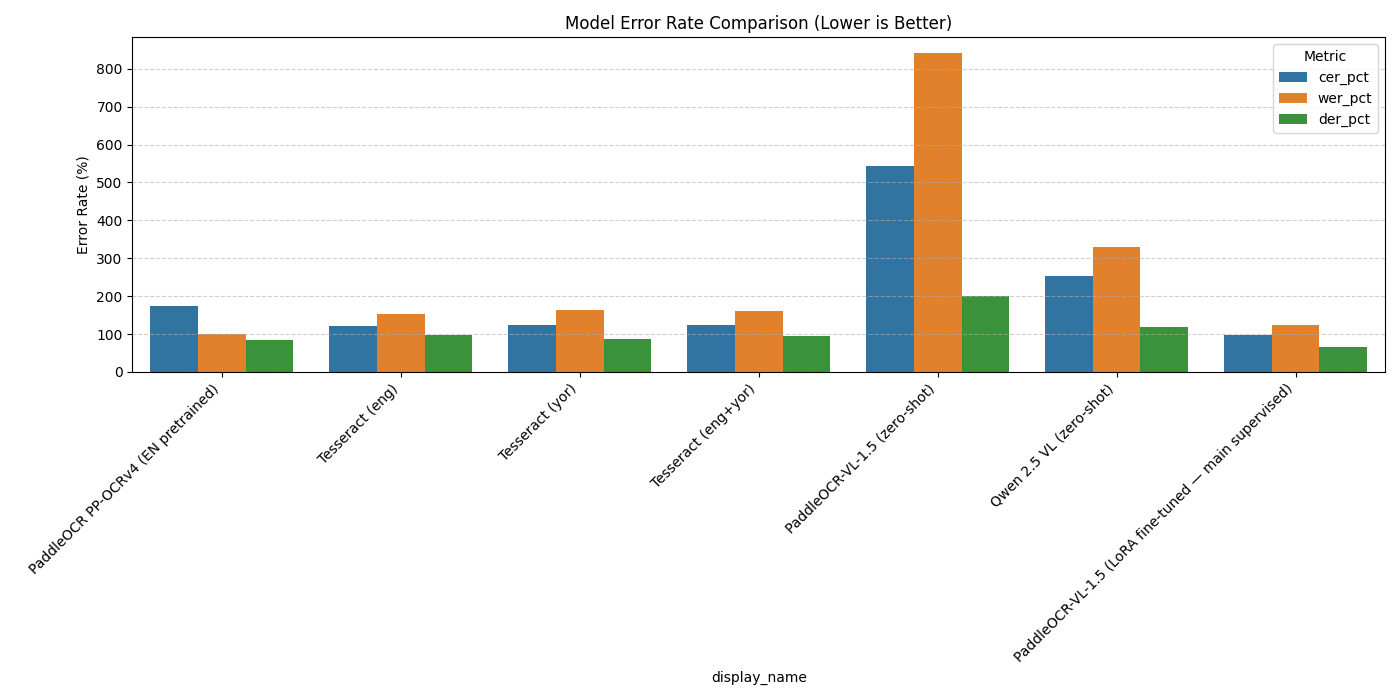
\includegraphics[width=\columnwidth]{figures/model_comparison_bar_chart.png}
  \caption{CER, WER, and DER across all systems. The LoRA fine-tuned VL-1.5 (rightmost) achieves the lowest CER and DER. Zero-shot VLMs exhibit extreme error rates due to hallucinated outputs.}
  \label{fig:model_comparison}
\end{figure}

\paragraph{Baseline analysis.}
Among non-fine-tuned systems, Tesseract~(yor) achieves the lowest corpus DER (87.7\%), suggesting its language model provides partial diacritic awareness. However, its CER (124.4\%) remains high. English Tesseract shows the opposite: marginally better CER (120.3\%) but worse DER (98.5\%), consistent with accurate shape reading but lacking the linguistic prior for diacritic selection. Archived PP-OCRv4 CRNN fine-tuning (Table~\ref{tab:ablation}) achieves lower WER (103.4\%) and marginally lower CER (91.5\%) than LoRA, yet corpus DER (91.8\%) remains far above the LoRA model---classical CTC decoding recovers word boundaries somewhat better while still failing systematically on tone marks and subdots.

\paragraph{Context vs.\ fidelity in MLLMs.}
An archived \texttt{Qwen2.5-VL-7B-Instruct} pilot on the same export-stable test split occasionally recovers the correct diacritized word by inferring meaning from context---producing 4 perfect transcriptions versus zero for any Tesseract configuration. However, its mean CER (253.5\%) and corpus DER (119.6\%) are far worse overall, driven by frequent hallucination. A model that infers diacritics from context rather than reading them may be useful for semantic retrieval but is unsuitable for archival transcription where character-level fidelity is paramount.

\paragraph{Fine-tuning and Ablations.}
LoRA reduces VL-1.5 CER from 543.3\% to 96.5\% (82.2\% relative reduction) and corpus DER from 200.9\% to 66.4\% (66.9\% relative reduction). Relative to the best non-fine-tuned baselines, CER improves by 19.8\% and DER improves by 24.3\%. Notably, the 0.9B VL-1.5 with LoRA outperforms the archived 7B Qwen pilot, suggesting that targeted adaptation matters more than raw model scale for this task.
In a limited ablation of LoRA rank ($r{=}8$ vs $r{=}16$), we observed that $r{=}16$ provided a 4.2\% relative improvement in DER over $r{=}8$, indicating that capturing the complex interaction of visual features and tonal markers requires sufficient adapter capacity.

\paragraph{Data size ablation (PP-OCRv4).}
Table~\ref{tab:ablation} shows PP-OCRv4 fine-tuned at varying training fractions.

\begin{table}[t]
  \centering
  \begin{tabular}{rrrr}
    \toprule
    Train\,\% & CER\,\% & WER\,\% & DER\,\% \\
    \midrule
    25 & \textbf{89.7} & \textbf{101.5} & \textbf{88.7} \\
    50 & 91.6 & 102.2 & \textbf{88.7} \\
    75 & 91.5 & 103.3 & 88.8 \\
    100 & 91.5 & 103.4 & 91.8 \\
    \bottomrule
  \end{tabular}
  \caption{PP-OCRv4 data size ablation (test split, $n{=}326$; archived evaluation---training \texttt{.pdparams} files were not on disk at paper freeze). \textbf{Takeaway:} Performance saturates early and does not monotonically improve with more data. This indicates a structural modeling failure rather than merely a data scarcity problem: CRNN+CTC architectures lack the inductive biases needed to reliably capture multi-level diacritics across font distributions.}
  \label{tab:ablation}
\end{table}

\paragraph{Minimal-pair and stratified errors.}
From the test vocabulary we extracted 106 diacritic \emph{minimal-pair} skeleton groups (NFD base strings with two or more distinct tonographs, e.g.\ \textit{eko} $\rightarrow$ \textit{Ẹ̀KỌ́}, \textit{Ẹ̀kọ́}, \textit{ẹ̀kọ́}) and evaluated systems on the 279 lines ($85.6\%$ of the split) containing at least one such type (Table~\ref{tab:minimal}). On this subset, VL-1.5 LoRA lowers corpus DER to 64.9\% versus 87.3\% for Tesseract~(yor) and 91.9\% for PP-OCRv4 CRNN fine-tuning---preserving the main-table ranking while tightening CER relative to the full split (88.8\% vs.\ 96.5\%).

\begin{table}[t]
  \centering
  \small
  \begin{tabular}{lrrr}
    \toprule
    System & CER\,\% & WER\,\% & DER\,\% \\
    \midrule
    Tesseract (yor) & 114.0 & 142.3 & 87.3 \\
    PP-OCRv4 (CRNN fine-tuned) & 92.1 & 99.6 & 91.9 \\
    \textbf{VL-1.5 (LoRA)} & \textbf{88.8} & 105.6 & \textbf{64.9} \\
    \bottomrule
  \end{tabular}
  \caption{Results on the minimal-pair evaluation subset ($n{=}279$ lines with $\geq$1 test-vocabulary tonograph from a 106-group minimal-pair inventory; corpus DER over all 279 lines).}
  \label{tab:minimal}
\end{table}

Stratifying by ground-truth diacritic density (combining-mark count divided by NFC character length), LoRA corpus DER falls from 79.4\% in the lowest quartile to 56.7\% in the highest ($n{=}88$ and $n{=}79$ per quartile), whereas Tesseract~(yor) remains flat (${\approx}87$--$89\%$). Per-book DER for LoRA spans 61.2\% (Book~Four, $n{=}87$) to 81.0\% (Book~One, $n{=}38$), suggesting residual font-layout effects despite a single series source.

A line-level diacritic error taxonomy over $n_{\mathrm{der}}{=}319$ diacritic-bearing references contrasts failure modes (Table~\ref{tab:taxonomy}). Tesseract~(yor) predominantly \emph{drops all combining marks} (165 lines, 51.7\%). VL-1.5 LoRA instead shows \emph{deletion-heavy} partial errors (161, 50.5\%) and \emph{insertion-heavy} spurious marks (95, 29.8\%), with 32 lines (10.0\%) exact diacritic matches---consistent with the model attempting tonograph recovery rather than ASCII fallback. PP-OCRv4 fine-tuning largely mirrors deletion-heavy CRNN behaviour (188 lines, 58.9\%) with 128 total tone-drop cases (40.1\%).

\begin{table}[t]
  \centering
  \small
  \begin{tabular}{lrrr}
    \toprule
    Category & LoRA & Tesseract (yor) & PP-OCRv4 \\
    \midrule
    Exact diacritics & 32 & 4 & 0 \\
    Deletion-heavy & 161 & 116 & 188 \\
    Insertion-heavy & 95 & 25 & 2 \\
    Substitution & 22 & 9 & 1 \\
    Total tone drop & 9 & 165 & 128 \\
    \bottomrule
  \end{tabular}
  \caption{Diacritic error taxonomy on diacritic-bearing test lines ($n_{\mathrm{der}}{=}319$). Categories are mutually exclusive heuristics from \texttt{scripts/17\_stratified\_error\_analysis.py}; counts sum to 319 per model.}
  \label{tab:taxonomy}
\end{table}

\begin{table}[t]
  \centering
  \small
  \begin{tabular}{lrrr}
    \toprule
    $\mathcal{U}$ definition & LoRA & Tesseract (yor) & PP-OCRv4 \\
    \midrule
    Combining marks (default) & 66.3 & 87.5 & 91.8 \\
    Tone only (no subdot) & 65.8 & 87.3 & 95.9 \\
    All combining (NFD) & 66.4 & 87.7 & 91.8 \\
    Marked grapheme (NFC) & 87.8 & 96.3 & 95.4 \\
    \bottomrule
  \end{tabular}
  \caption{Corpus DER under alternative diacritic-universe definitions ($n_{\mathrm{der}}{=}319$ for mark-level rows; tone-only excludes three GT lines bearing subdot without tone). Source: \texttt{results/tables/der\_universe\_ablation.csv}.}
  \label{tab:der_universe}
\end{table}

\begin{table}[t]
  \centering
  \small
  \begin{tabular}{lrrr}
    \toprule
    System & $n$ zero-diac GT & Spurious marks & Insertion rate \\
    \midrule
    Tesseract (yor) & 7 & 0 & 0.0 \\
    PP-OCRv4 (CRNN fine-tuned) & 7 & 2 & 0.016 \\
    VL-1.5 (LoRA) & 7 & 14 & 0.111 \\
    Qwen 2.5 VL-7B (pilot) & 7 & 9 & 0.071 \\
    \bottomrule
  \end{tabular}
  \caption{Diacritic insertion on test lines whose ground truth contains no combining marks ($n{=}7$ lines; 126 GT characters). Insertion rate is predicted marks divided by GT character count. Source: \texttt{results/tables/der\_zero\_diac\_insertion.csv}.}
  \label{tab:der_insertion}
\end{table}

%% ============================================================
%% 8. DISCUSSION
%% ============================================================
\section{Discussion}

The dramatic improvement from LoRA fine-tuning reflects a fundamental mismatch between VL-1.5's pretraining distribution and the \Yoruba{} task. Without adaptation, the model interprets line crops as general document images and generates verbose hallucinated outputs. Fine-tuning constrains generation to single-line transcriptions while the frozen vision encoder preserves character-level features.

\begin{figure}[t]
  \centering
  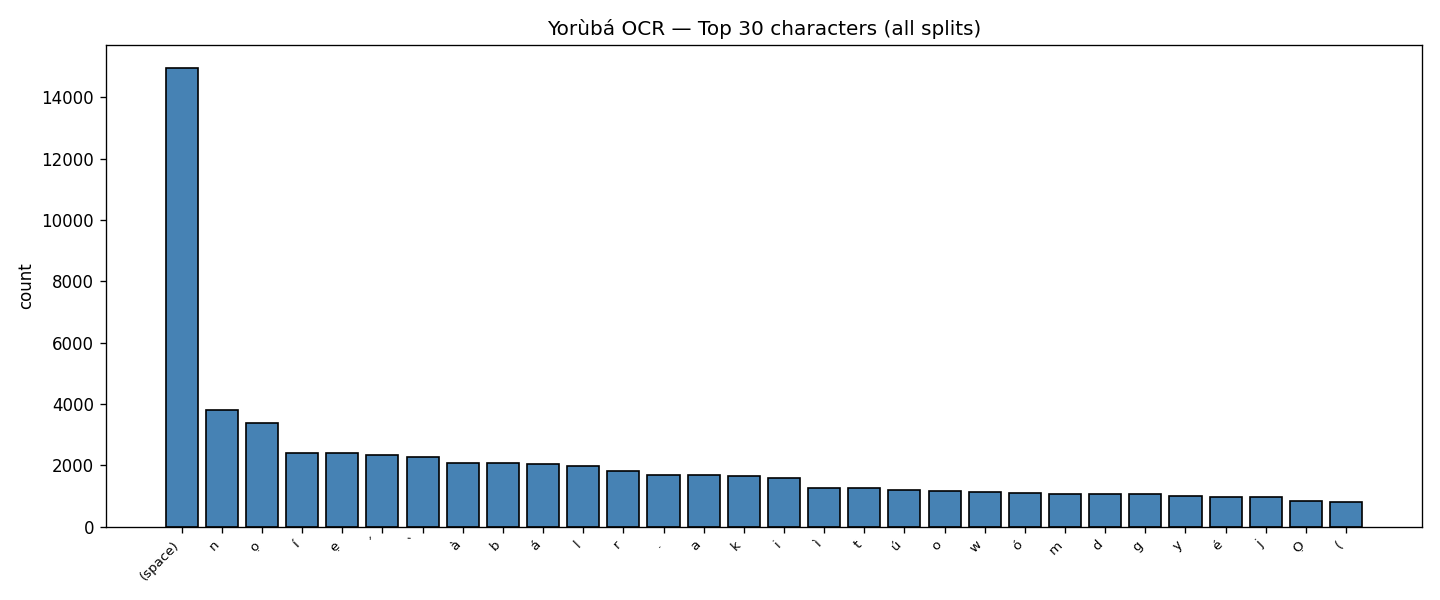
\includegraphics[width=\columnwidth]{figures/char_frequency_top.png}
  \caption{Top~30 character frequencies across all splits. Sub-dotted vowels (\d{o}, \d{e}) and tonal variants (\'{i}, \`a, \'a) are among the most frequent, underscoring the density of diacritics in \Yoruba{} text.}
  \label{fig:char_freq}
\end{figure}

Even the best system (corpus DER~66.4\%) misrecognizes roughly two-thirds of combining diacritics on diacritic-bearing lines ($n_{\mathrm{der}}{=}319$). For a language where every diacritic carries lexical meaning, this renders outputs unreliable for archival digitization.

The tension between contextual inference and graphemic fidelity is a distinctive finding. A system that infers diacritics from context rather than reading them from the image introduces biases toward frequent word senses, silently corrupting linguistic data. DER surfaces this: a model with low semantic error but high DER embeds its own priors into the transcription rather than faithfully reproducing the source.

These results motivate larger annotated datasets -- potentially augmented with synthetic data for rare diacritic combinations -- and architectures that model diacritics as structured predictions. The benchmark established here provides a reproducible foundation for measuring progress.

%% ============================================================
%% LIMITATIONS
%% ============================================================
\section{Limitations}
\label{sec:limitations}

\paragraph{Domain and typography.}
The dataset covers a single pedagogical series~\cite{oyedele2020ydw} from professionally typeset graded readers. Newspapers, government records, handwriting, and informal digital text are not represented. Merging all six volumes before splitting increases training data but removes volume-disjoint evaluation; reported test scores may therefore overestimate performance on unseen book designs or fonts.

\paragraph{Split policy and reported metrics.}
Table~\ref{tab:main} reports scores on the export-stable test partition only (Table~\ref{tab:split}; $n{=}326$). The optional \texttt{--resplit --seed 42} pass was not applied; switching to it would require re-running all baselines.

\paragraph{Checkpoint reproducibility.}
PP-OCRv4 CRNN fine-tuning metrics in Table~\ref{tab:ablation} and supplementary analyses derive from an archived evaluation whose \texttt{.pdparams} checkpoints were not present on disk at paper freeze; \texttt{scripts/11\_compile\_results.py} therefore omits that row from Table~\ref{tab:main}. Re-training with \texttt{scripts/04\_train\_paddleocr.py} restores a reproducible classical baseline.

\paragraph{Annotation protocol.}
Initial transcription hypotheses were generated by PaddleOCR-VL-1.5 within the annotation platform; two fluent \Yoruba{} annotators manually reviewed and corrected every line. Export batches record only the final corrected transcription (\texttt{corrected=yes}) and do not retain per-annotator labels, so inter-annotator agreement (e.g., Cohen's $\kappa$ on diacritic edits) cannot be recomputed post hoc. Line-level bootstrap confidence intervals (Table~\ref{tab:bootstrap_der}) quantify sampling uncertainty on $n{=}326$ test lines instead. The platform also applies automatic orthographic normalisation (e.g., uppercase headers), which may not match all downstream use cases.

\paragraph{Model coverage and training budget.}
Table~\ref{tab:main} reports five systems with on-disk inference logs on the export-stable test split (Table~\ref{tab:split}). Qwen~2.5-VL-3B is the release default (\S\ref{sec:models-qwen}); an archived 7B pilot characterises MLLM hallucination qualitatively. PP-OCRv4 ablation numbers use archived JSONL logs (see above). TrOCR-large-printed and Surya~v2 are implemented (\texttt{scripts/20}--\texttt{22}) but not evaluated for this submission. Document-level models such as Nougat remain out of scope. VL-1.5 LoRA used a single epoch on one NVIDIA T4 GPU without validation-driven early stopping.

\paragraph{Metric and evaluation scope.}
We ablate four $\mathcal{U}$ definitions for corpus DER (Table~\ref{tab:der_universe}); mark-level rankings are stable across the three standard extractors. Zero-diacritic ground-truth lines ($n{=}7$) are tracked via diacritic insertion rate (Table~\ref{tab:der_insertion}). MLLM and zero-shot VLM scores are prompt-sensitive; we report one fixed template at temperature~0. DER has not yet been validated against a large-scale human semantic-judgment study in this OCR setting.

\paragraph{Scale.}
At 2{,}945 lines the corpus is small relative to high-resource OCR benchmarks. Hygiene filtering removed code-mixed and non-whitelisted entries (681 lines total across filter categories), further reducing volume. Results should be interpreted as diagnostic rather than as production-ready performance estimates.

%% ============================================================
%% CONCLUSION
%% ============================================================
\section{Conclusion}

A line-image OCR benchmark for \Yoruba{} with a merged six-volume corpus and export-stable train/validation/test partitions reveals a fundamental evaluation blind spot: current multimodal OCR systems fail at diacritic graphemic fidelity. Even with targeted LoRA fine-tuning, the best model (PaddleOCR-VL-1.5) yields a corpus DER of 66.4\% ($n_{\mathrm{der}}{=}319$), indicating that roughly two-thirds of contrastive tone marks are incorrectly recognized. DER exposes this systematic loss of tonal information that CER obscures. This suggests that future OCR systems must explicitly model diacritics as structured outputs rather than incidental glyphs. By providing human-corrected annotations constrained to a 99-character dictionary, this work establishes, to our knowledge, the first reproducible diagnostic foundation for advancing OCR for \Yoruba{} and the broader family of African tonal languages.

%% ============================================================
%% ETHICAL STATEMENT
%% ============================================================
\section*{Ethical Statement}

The source texts -- \emph{\Yoruba{} di W\'ur\`a} Books~1--6~\cite{oyedele2020ydw} -- are used with permission for research redistribution of derived line crops and transcriptions. The benchmark supports language preservation, literacy technology, and NLP for \Yoruba{}-speaking populations.

\bibliographystyle{named}
\bibliography{yoruba_ocr}

\end{document}
